\chapter{フェーズ①' JavaScript で動きをつける}
\sheet{8-1〜8-12}

第7章のページは、見た目は整いましたが、まだ何も「動き」ません。
この章では JavaScript を使って、次の2つを作ります。

\begin{center}
\fcolorbox{gray!50}{white}{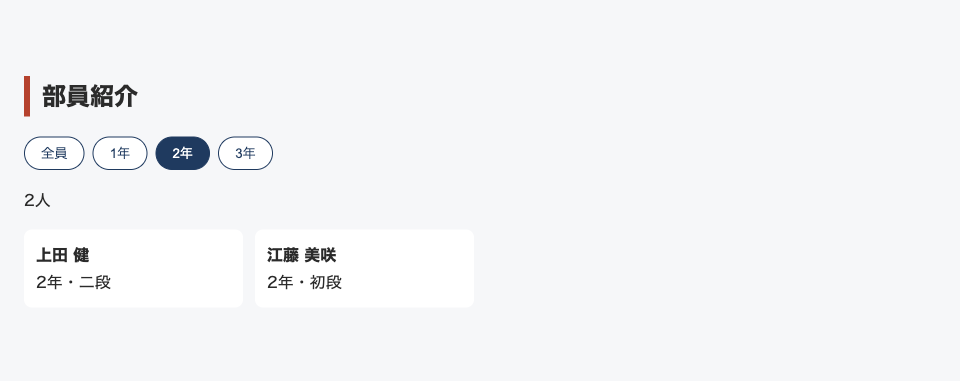
\includegraphics[width=0.47\linewidth]{js-members.png}}\hfill
\fcolorbox{gray!50}{white}{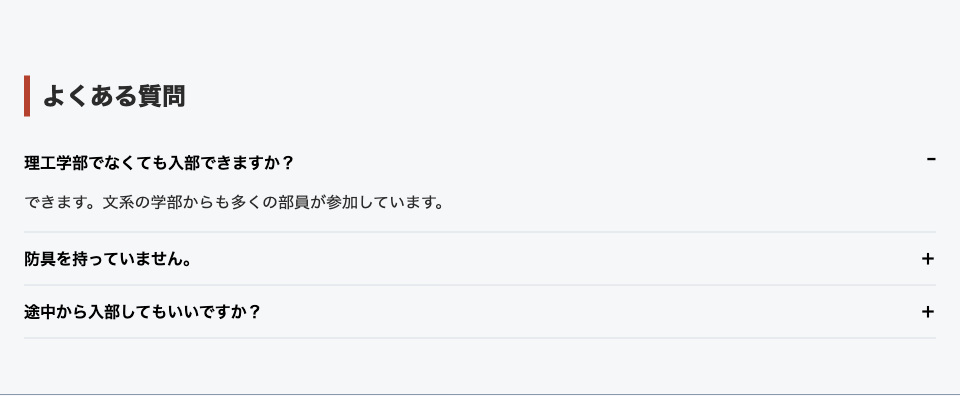
\includegraphics[width=0.47\linewidth]{js-faq.png}}
\end{center}
\figcap{左：学年のボタンで部員を絞り込む　右：質問を押すと答えが開く}

どちらも、\textbf{データ（配列）を用意して、そこから画面を作る}という形で作ります。
これは、第2巻の React でも、第3巻のデータベースでも、本番のサイトでも、ずっと同じ形です。
この章で一番身につけてほしい考え方です。

\section{JavaScript を動かしてみる}

JavaScript は、ブラウザの中で動くプログラミング言語です。
まずはファイルを作らずに、ブラウザの\term{コンソール}で動かしてみます。

\begin{step}{コンソールで計算する}
\sheet{8-1}
ブラウザで \key{F12} を押し、開発者ツールの \menu{Console} タブを開きます。
\code{>} の横に次のように打ち、\key{Enter} を押します。
\begin{terminal}[Console]
> 1 + 2
3
> "面" + "打ち"
'面打ち'
> console.log("稽古開始")
稽古開始
\end{terminal}
\end{step}

\begin{tip}[貼り付けが拒否されたら]
コンソールに初めてコードを貼り付けると、安全のために「allow pasting と入力してください」と表示されることがあります。
これは、知らない人に言われるままコードを貼って乗っ取られる詐欺を防ぐための仕組みです。
この教材のコードは自分で打つので、表示された通りに入力して進めてかまいません。
\end{tip}

\section{変数とデータの型}

\term{変数}は、値に名前をつけて取っておく箱です。

\begin{Piton}[language=code]
const clubName = "理工体剣道部";   // 変えない値は const
let count = 0;                     // あとで変える値は let
count = count + 1;
console.log(clubName, count);      // → 理工体剣道部 1
\end{Piton}

\begin{tip}[const と let の使い分け]
\textbf{基本は \code{const}}、あとで値を入れ直すときだけ \code{let} を使います。
古い資料に出てくる \code{var} は使いません。
\end{tip}

\begin{center}\small
\begin{tabularx}{\linewidth}{l l X}
\toprule
型 & 例 & 説明 \\
\midrule
文字列（string） & \code{"面"}、\code{'小手'} & 文字。\code{"} か \code{'} で囲む \\
数値（number） & \code{4}、\code{18.5} & 計算できる数 \\
真偽値（boolean） & \code{true}、\code{false} & はい／いいえ \\
配列（array） & \code{["面", "小手", "胴"]} & 値の並び。順番がある \\
オブジェクト（object） & \code{\{ name: "上田", grade: 2 \}} & 名前付きの値のまとまり \\
\bottomrule
\end{tabularx}
\end{center}

\begin{caution}["2" と 2 は別物]
\code{"2"} は文字列、\code{2} は数値です。見た目は同じでも、\code{"2" === 2} は \code{false} になります。
画面のボタンから取り出した値はたいてい文字列なので、数値と比べるときは \code{Number("2")} で数値に変換します。
この章の絞り込みで、実際にこの変換が出てきます。
\end{caution}

\section{配列とオブジェクト}

部員1人分の情報は、オブジェクトで表せます。部員全員は、それを並べた配列で表せます。

\begin{Piton}[language=code]
const members = [
  { name: "青木 太郎", grade: 3, dan: "三段", role: "主将" },
  { name: "上田 健",   grade: 2, dan: "二段", role: "" },
];

console.log(members.length);     // → 2（人数）
console.log(members[0].name);    // → 青木 太郎（0 番目の人の名前）
console.log(members[1].grade);   // → 2
\end{Piton}

\begin{why}[配列は 0 番から数える]
配列の最初の要素は \code{[0]}、2番目は \code{[1]} です。最初は戸惑いますが、ほぼすべてのプログラミング言語がこの数え方です。
\end{why}

この「オブジェクトの配列」は、データベースの表とそっくりです。

\begin{center}
\begin{tikzpicture}[font=\sffamily\scriptsize]
  \node[draw=kon,fill=white,align=left,font=\ttfamily\scriptsize,inner sep=6pt] (js) {[\\
  \ \ \{ name: "青木", grade: 3 \},\\
  \ \ \{ name: "上田", grade: 2 \},\\
  ]};
  \node[right=1.8cm of js] (tb) {\begin{tabular}{|l|l|}\hline \rowcolor{kon!15} name & grade\\\hline 青木 & 3\\\hline 上田 & 2\\\hline\end{tabular}};
  \draw[{Stealth}-{Stealth},thick,gray] (js) -- node[above]{同じ形} (tb);
  \node[below=1mm of js] {JavaScript の配列};
  \node[below=1mm of tb] {データベースの表（第3巻）};
\end{tikzpicture}
\end{center}

\section{関数}

\term{関数}は、処理に名前をつけて、何度でも呼び出せるようにしたものです。

\begin{Piton}[language=code]
// 受け取った部員の紹介文を返す関数
function introduce(member) {
  return `${member.grade}年の${member.name}です`;
}

console.log(introduce(members[0]));   // → 3年の青木 太郎です

// 同じ関数を「アロー関数」で書くと、こうなる
const introduce2 = (member) => `${member.grade}年の${member.name}です`;
\end{Piton}

\code{`}（バッククォート）で囲んだ文字列は\term{テンプレートリテラル}といい、\code{\$\{ \}} の中に変数を埋め込めます。
\key{Shift}+\key{@} で入力できます。

\section{条件分岐と繰り返し}

\begin{Piton}[language=code]
// if：条件によって処理を分ける
const member = members[0];
if (member.role === "主将") {
  console.log("主将です");
} else {
  console.log("部員です");
}

// forEach：配列の1人ずつに同じ処理をする
members.forEach((member) => {
  console.log(member.name);
});
\end{Piton}

\begin{tip}[=== を使う]
「等しいか」を調べるときは \code{===}（イコール3つ）を使います。\code{==}（2つ）は型を勝手に変換して比べるので、思わぬ結果になることがあります。
\end{tip}

\section{配列を変換する：filter と map}

この章で一番大事な2つの道具です。

\begin{center}
\begin{tikzpicture}[font=\sffamily\scriptsize,
  item/.style={draw,rounded corners=2pt,minimum width=1.3cm,minimum height=0.55cm,fill=white},
  arr/.style={-{Stealth},thick}]
  \node[font=\sffamily\small\bfseries] at (-1.6,1.2) {filter};
  \foreach \i/\g in {0/3,1/3,2/2,3/2,4/1}{ \node[item] at (\i*1.5,1.2) {\g 年}; }
  \foreach \i/\g in {0/2,1/2}{ \node[item,draw=shu] at (\i*1.5+2.25,0) {\g 年}; }
  \draw[arr,shu] (3,0.85) -- node[right]{\texttt{m => m.grade === 2}} (3,0.35);
  \node[anchor=west] at (6.5,0) {条件に合うものだけ残す};

  \node[font=\sffamily\small\bfseries] at (-1.6,-1.2) {map};
  \foreach \i/\n in {0/青木,1/上田}{ \node[item] at (\i*3+0.75,-1.2) {\n}; }
  \foreach \i/\n in {0/青木,1/上田}{ \node[item,draw=matcha,minimum width=2.6cm,font=\ttfamily\tiny] at (\i*3+0.75,-2.4) {<li>\n</li>}; }
  \draw[arr,matcha] (2.25,-1.55) -- node[right]{1つずつ形を変える} (2.25,-2.05);
  \node[anchor=west] at (6.5,-2.4) {同じ数の、変換後の配列を作る};
\end{tikzpicture}
\end{center}

\begin{Piton}[language=code]
// 2年生だけを取り出す
const second = members.filter((member) => member.grade === 2);

// 名前だけの配列にする
const names = members.map((member) => member.name);   // → ["青木 太郎", "上田 健"]

// HTML の文字列に変換して、つなげる
const html = members.map((member) => `<li>${member.name}</li>`).join("");
\end{Piton}

\section{DOM：JavaScript から HTML を操作する}

ブラウザは、読み込んだ HTML を\term{DOM}という「木」の形で覚えています。
JavaScript はこの木の枝を探して、中身を書き換えたり、クリックを待ち受けたりできます。

\begin{center}\small
\begin{tabularx}{\linewidth}{>{\ttfamily}l X}
\toprule
\normalfont 書き方 & すること \\
\midrule
document.querySelector(".a") & CSS と同じ書き方で、最初に見つかった1つの要素を取ってくる \\
document.querySelectorAll(".a") & 当てはまる要素を全部取ってくる \\
要素.textContent = "..." & 中の文字を書き換える \\
要素.innerHTML = "..." & 中の HTML を書き換える \\
要素.classList.add("x") & class を足す（\code{remove} で外す、\code{toggle} で付け外しを切り替える） \\
要素.addEventListener("click", 関数) & クリックされたら関数を実行する \\
要素.dataset.grade & HTML の \code{data-grade="2"} の値を取り出す \\
\bottomrule
\end{tabularx}
\end{center}

\section{作ってみる}

\begin{step}{HTML に部員紹介の枠を足し、JavaScript を読み込む}
\sheet{8-6}
\code{kendo-top} の \code{index.html} で、「よくある質問」のセクションを、次の2つのセクションに\textbf{置き換えます}。
質問と答えは、HTML に直接書くのをやめ、JavaScript のデータから作ります。
\begin{filebox}{index.html（「よくある質問」のセクションを置き換え）}
\begin{Piton}[language=code]
    <section id="members" class="section">
      <h2>部員紹介</h2>
      <div class="filter">
        <button class="filter-button is-active" data-grade="all">全員</button>
        <button class="filter-button" data-grade="1">1年</button>
        <button class="filter-button" data-grade="2">2年</button>
        <button class="filter-button" data-grade="3">3年</button>
      </div>
      <p class="member-count"></p>
      <ul class="member-list"></ul>
    </section>

    <section id="faq" class="section">
      <h2>よくある質問</h2>
      <div class="faq-list"></div>
    </section>
\end{Piton}
\end{filebox}
さらに、\code{</body>} の直前に次の2行を足します。
\begin{filebox}{index.html（</body> の直前）}
\begin{Piton}[language=code]
  <script src="data.js"></script>
  <script src="script.js"></script>
\end{Piton}
\end{filebox}
\end{step}

\begin{why}[script を body の最後に置く理由]
ブラウザは HTML を上から順に読みます。
\code{<script>} を \code{<head>} に置くと、まだ部員紹介の枠（\code{.member-list}）が作られる前に JavaScript が動いてしまい、
「枠が見つからない」というエラーになります。一番最後に置けば、枠ができあがった後に動きます。
\end{why}

\begin{step}{データのファイルを作る}
\sheet{8-7}
\begin{filebox}{data.js}
\begin{Piton}[language=code]
// 部員のデータ（名前はダミー）
const members = [
  { name: "青木 太郎", grade: 3, dan: "三段", role: "主将" },
  { name: "井上 花子", grade: 3, dan: "二段", role: "女子主将" },
  { name: "上田 健", grade: 2, dan: "二段", role: "" },
  { name: "江藤 美咲", grade: 2, dan: "初段", role: "" },
  { name: "小川 翔", grade: 1, dan: "無", role: "" },
  { name: "加藤 葵", grade: 1, dan: "初段", role: "" },
];

// よくある質問のデータ
const faqs = [
  {
    question: "理工学部でなくても入部できますか？",
    answer: "できます。文系の学部からも多くの部員が参加しています。",
  },
  {
    question: "防具を持っていません。",
    answer: "部の貸し出し用があります。慣れてから自分のものを買う人がほとんどです。",
  },
  {
    question: "途中から入部してもいいですか？",
    answer: "もちろんです。秋から入部する人もいます。",
  },
];
\end{Piton}
\end{filebox}
\textbf{名前はダミーです。}このリポジトリは公開されるので、本物の部員の名前は入れません。
\end{step}

\begin{why}[データと処理を別のファイルに分ける理由]
部員が入れ替わったときに直すのは \code{data.js} だけで済み、処理の \code{script.js} には触らずに済みます。
本番のサイトでは、このデータの置き場所がデータベースになり、管理画面から書き換えられるようになります。
「データと処理を分ける」という考え方が、そのまま本番の仕組みにつながっています。
\end{why}

\begin{step}{よくある質問を作り、クリックで開閉させる}
\sheet{8-8}
\begin{filebox}{script.js}
\begin{Piton}[language=code]
// ===== よくある質問：データから HTML を作り、クリックで開閉する =====
const faqList = document.querySelector(".faq-list");

faqs.forEach((faq) => {
  const item = document.createElement("div");
  item.className = "faq-item";
  item.innerHTML = `
    <button class="faq-question">${faq.question}</button>
    <p class="faq-answer">${faq.answer}</p>
  `;
  faqList.appendChild(item);
});

const questionButtons = document.querySelectorAll(".faq-question");

questionButtons.forEach((button) => {
  button.addEventListener("click", () => {
    const item = button.parentElement;
    item.classList.toggle("is-open");
  });
});

\end{Piton}
\end{filebox}
1行ずつ読むと、次のことをしています。
\begin{enumerate}
  \item \code{.faq-list} の枠を取ってくる
  \item \code{faqs} の1つずつについて、\code{div} を作り、中に質問のボタンと答えの段落を入れて、枠に足す
  \item できあがった質問のボタンを全部取ってくる
  \item それぞれのボタンに「押されたら、親の \code{div} の \code{is-open} を付け外しする」という仕掛けをつける
\end{enumerate}
開いた・閉じたの見た目は、次の STEP の CSS で \code{is-open} が付いているかどうかによって切り替えます。
\textbf{JavaScript は class を付け外しするだけ、見た目は CSS に任せる}、という役割分担です。
\end{step}

\begin{step}{部員紹介を作り、学年で絞り込む}
\sheet{8-9}
\code{script.js} の続きに書きます。
\begin{filebox}{script.js（続き）}
\begin{Piton}[language=code]
// ===== 部員紹介：学年で絞り込む =====
const memberList = document.querySelector(".member-list");
const memberCount = document.querySelector(".member-count");
const filterButtons = document.querySelectorAll(".filter-button");

function renderMembers(grade) {
  // "all" なら全員、それ以外は学年が一致する人だけ残す
  const shown =
    grade === "all"
      ? members
      : members.filter((member) => member.grade === Number(grade));

  memberList.innerHTML = shown
    .map((member) => {
      const role = member.role ? `<span class="role">${member.role}</span>` : "";
      return `<li class="member">${role}<strong>${member.name}</strong><br>${member.grade}年・${member.dan}</li>`;
    })
    .join("");

  memberCount.textContent = `${shown.length}人`;
}

filterButtons.forEach((button) => {
  button.addEventListener("click", () => {
    filterButtons.forEach((b) => b.classList.remove("is-active"));
    button.classList.add("is-active");
    renderMembers(button.dataset.grade);
  });
});

// 最初は全員を表示する
renderMembers("all");
\end{Piton}
\end{filebox}
\code{renderMembers} は「学年を受け取って、その学年の部員で画面を描き直す」関数です。
ボタンが押されるたびに、押されたボタンの \code{data-grade} を渡して呼び出しています。
\code{data-grade} の値は文字列なので、\code{Number(grade)} で数値に変換してから \code{member.grade} と比べています。
\end{step}

\begin{step}{CSS を足す}
\sheet{8-10}
\code{style.css} の \code{/* よくある質問 */} のルール（\code{.faq dt} と \code{.faq dd}）を消して、代わりに次を足します。
\begin{filebox}{style.css}
\begin{Piton}[language=code]
/* 部員紹介 */
.filter {
  display: flex;
  gap: 8px;
}

.filter-button {
  padding: 6px 16px;
  border: 1px solid var(--color-kon);
  border-radius: 999px;
  background-color: white;
  color: var(--color-kon);
  cursor: pointer;
}

.filter-button.is-active {
  background-color: var(--color-kon);
  color: white;
}

.member-list {
  display: grid;
  grid-template-columns: repeat(auto-fill, minmax(180px, 1fr));
  gap: 12px;
  padding: 0;
  list-style: none;
}

.member {
  padding: 12px;
  background-color: white;
  border-radius: 8px;
}

.role {
  display: inline-block;
  margin-right: 6px;
  padding: 0 8px;
  border-radius: 4px;
  background-color: var(--color-shu);
  color: white;
  font-size: 12px;
}

/* よくある質問（開閉） */
.faq-item {
  border-bottom: 1px solid #d9dde3;
}

.faq-question {
  width: 100%;
  padding: 14px 0;
  border: none;
  background: none;
  text-align: left;
  font-size: 16px;
  font-weight: bold;
  cursor: pointer;
}

.faq-question::after {
  content: "＋";
  float: right;
}

.faq-answer {
  display: none;
  margin-top: 0;
}

.faq-item.is-open .faq-answer {
  display: block;
}

.faq-item.is-open .faq-question::after {
  content: "−";
}

\end{Piton}
\end{filebox}
\code{display: grid;} は Flexbox の仲間で、\textbf{縦横のマス目}に並べるときに使います。
\code{repeat(auto-fill, minmax(180px, 1fr))} は「1マス最低 180px で、入るだけ並べる」という意味で、
メディアクエリを書かなくても画面幅に合わせて列の数が自動で変わります。
\end{step}

ブラウザで動きを確かめたら、コミットして push します。

\begin{terminal}[Git Bash]
$ git add index.html data.js script.js style.css
$ git commit -m "feat: よくある質問の開閉と、部員の学年絞り込みを追加"
$ git push
\end{terminal}

\section{エラーの読み方}

JavaScript でつまずいたら、まず開発者ツールの \menu{Console} を見ます。赤い文字がエラーです。

\begin{terminal}[Console]
Uncaught TypeError: Cannot read properties of null (reading 'appendChild')
    at script.js:11:11
\end{terminal}

\begin{center}\small
\begin{tabularx}{\linewidth}{l X}
\toprule
部分 & 読み方 \\
\midrule
\code{TypeError} & エラーの種類。「型が想定と違う」 \\
\code{Cannot read properties of null} & 「\code{null}（何もない）の中身を読もうとした」 \\
\code{(reading 'appendChild')} & 読もうとしたのは \code{appendChild} \\
\code{script.js:11:11} & \textbf{\code{script.js} の11行目}。クリックするとその場所が開く \\
\bottomrule
\end{tabularx}
\end{center}

つまり、「11行目で \code{appendChild} しようとした相手が \code{null}（見つからなかった）」ということです。
よくある原因は、\code{querySelector} に渡したクラス名の打ち間違い（\code{.faq-lsit} など）か、
\code{<script>} を置く場所が早すぎることです。

\begin{center}\small
\begin{tabularx}{\linewidth}{>{\ttfamily\raggedright\arraybackslash}p{5.5cm} X}
\toprule
\normalfont よく出るエラー & よくある原因 \\
\midrule
X is not defined & 変数名の打ち間違い。大文字と小文字も区別される \\
Cannot read properties of null & \code{querySelector} で要素が見つかっていない \\
Cannot read properties of undefined & 配列の範囲外（\code{members[10]}）や、存在しない名前（\code{member.nmae}）を読んだ \\
Unexpected token & かっこやカンマの閉じ忘れ・付けすぎ \\
X is not a function & 関数でないものを \code{()} で呼んだ。名前の打ち間違いが多い \\
\bottomrule
\end{tabularx}
\end{center}

\begin{prompt}[エラーを Claude に聞くとき]
script.js を実行したら、コンソールにこのエラーが出た。\\
（エラーを全文貼る）\\
私は、11行目の faqList が null になっているのが原因だと思っている。この読みが合っているかと、なぜ null になるのかを教えて。直したコードはまだ出さないで。
\end{prompt}

\section{練習問題}
\sheet{8-13〜8-24}

\code{\textasciitilde/dev/js-drill} フォルダを作り、問題ごとにファイル（\code{q01.js} など）を分けて解きます。
1〜9 は、\code{node q01.js} のように Git Bash で実行して結果を確かめられます（Node.js は第3章で入れました）。
10〜12 は HTML と組み合わせるので、ブラウザで確かめます。

\begin{tip}[node で実行する]
\begin{terminal}[Git Bash]
$ cd ~/dev/js-drill
$ node q01.js
\end{terminal}
\code{console.log} で出したものが、そのままターミナルに表示されます。
\end{tip}

\subsection*{基本}

\begin{exercise}[1]{稽古の合計時間}
\toanswer\par
1回の稽古が120分、週に4回、前期が15週あります。前期の稽古時間の合計を「分」で計算して表示してください。
数字はすべて \code{const} の変数に入れ、計算式の中に数字を直接書かないこと。
\end{exercise}

\begin{exercise}[1]{型を当てる}
\toanswer\par
次のそれぞれを \code{console.log} すると何が表示されるか、\textbf{先に予想を書いてから}実行してください。
\begin{Piton}[language=code]
console.log(typeof "4");
console.log(typeof 4);
console.log("4" + 4);
console.log(4 + 4);
console.log("4" === 4);
console.log(Number("4") === 4);
\end{Piton}
\end{exercise}

\begin{exercise}[1]{技の配列}
\toanswer\par
\code{["面", "小手", "胴"]} という配列を作り、次の順に操作して、そのたびに配列全体と長さを表示してください。
(1) 最後に \code{"突き"} を足す　(2) 2番目の要素（\code{"小手"}）だけを表示する　(3) 最後の要素を、長さを使って取り出す
\end{exercise}

\begin{exercise}[1]{自分のプロフィール}
\toanswer\par
自分の名前・学年・学科・好きな技をオブジェクトにまとめ、テンプレートリテラルを使って
「応用化学科2年の柴山です。好きな技は出小手です。」のような文を表示してください。
\end{exercise}

\begin{exercise}[2]{分を「時間と分」に直す関数}
\toanswer\par
分を受け取って、\code{"2時間30分"} のような文字列を返す関数 \code{formatMinutes} を作ってください。
\code{formatMinutes(150)} → \code{"2時間30分"}、\code{formatMinutes(60)} → \code{"1時間0分"}、\code{formatMinutes(45)} → \code{"0時間45分"}。
（ヒント：割り算の余りは \code{\%}、小数の切り捨ては \code{Math.floor}）
余裕があれば、\code{"1時間"}、\code{"45分"} のように0の部分を省略するようにしてください。
\end{exercise}

\begin{exercise}[2]{上級生と下級生}
\toanswer\par
学年を受け取り、1年なら \code{"新入生"}、2年なら \code{"中堅"}、3年以上なら \code{"上級生"}、
それ以外（0 や負の数）なら \code{"学年が正しくありません"} を返す関数を作り、5つの値で試してください。
\end{exercise}

\subsection*{配列の変換}

以下の問題では、本章の \code{data.js} の \code{members} を、ファイルの先頭にコピーして使います。

\begin{exercise}[2]{段位を持っている人}
\toanswer\par
段位が \code{"無"} でない部員だけを取り出し、その人数と名前を表示してください。
\end{exercise}

\begin{exercise}[2]{さん付けの名簿}
\toanswer\par
\code{map} を使って、\code{["青木 太郎さん（3年）", "井上 花子さん（3年）", ...]} という配列を作ってください。
次に、\code{join} を使って、それを改行区切りの1つの文字列にして表示してください。
\end{exercise}

\begin{exercise}[3]{学年ごとの人数}
\toanswer\par
学年ごとの人数を数え、\code{\{ 1: 2, 2: 2, 3: 2 \}} のようなオブジェクトを作って表示してください。
学年が増えても（4年がいても）コードを書き換えずに済むようにすること。
\end{exercise}

\subsection*{画面を動かす}

\begin{exercise}[2]{素振りカウンター}
\toanswer\par
「素振り +1」ボタンと「リセット」ボタン、回数を表示する場所を作ってください。
「+1」を押すたびに回数が1ずつ増え、100回になったら文字の色が朱色に変わるようにします。
（ヒント：色は JavaScript で直接変えず、CSS の class を付け外しする）
\end{exercise}

\begin{exercise}[3]{名前で検索する}
\toanswer\par
本章の部員紹介に、名前の検索欄（\code{<input type="text">}）を足してください。
文字を打つたびに、その文字を名前に含む部員だけが表示されるようにします。
（ヒント：\code{input} イベントと、文字列の \code{includes}）
\end{exercise}

\begin{exercise}[3]{バグを直す}
\toanswer\par
次のコードは、2年生の名前だけを画面に表示するつもりで書かれていますが、\textbf{バグが3つ}あります。
コンソールのエラーを読みながら、すべて直してください。直した理由もそれぞれ1行で書きます。
\begin{filebox}{q12.js}
\begin{Piton}[language=code]
const list = document.querySelector(".member-lsit");
const grade = "2";

const second = members.filter((member) => member.grade === grade);

list.innerHTML = second.map((member) => `<li>${member.nmae}</li>`).join("");
\end{Piton}
\end{filebox}
\end{exercise}


\begin{challenge}{部員紹介に「役職」と「段位」の絞り込みを足す}
\sheet{8-25}
\begin{enumerate}
  \item 学年のボタンの下に、「役職のある人だけ」というチェックボックスを付ける。チェックを入れると、役職（\code{role}）が空でない人だけが表示される
  \item \textbf{学年とチェックボックスは同時に効く}こと（例：3年 ＋ 役職のある人だけ → 主将と女子主将の2人）
  \item 並び順を「学年の高い順、同じ学年なら名前順」にする（ヒント：\code{sort}）
  \item \code{data.js} にダミーの部員を4人足し、表示や人数が正しく変わることを確かめる
\end{enumerate}
\textbf{手を動かす前に}、「\code{renderMembers} のどこを、どう変えれば、2つの条件を同時に効かせられるか」をメモに書いてください。
定例では、そのメモと実際のコードを並べて説明します。
\end{challenge}

\begin{checklist}
\begin{itemize}
  \checkitem \code{const} と \code{let} を使い分けられる
  \checkitem 文字列の \code{"2"} と数値の \code{2} が違うことを説明できる
  \checkitem オブジェクトの配列から、\code{filter} と \code{map} で必要な形を作れる
  \checkitem \code{querySelector} と \code{addEventListener} で、クリックに反応させられる
  \checkitem 「JavaScript は class を付け外しするだけ、見た目は CSS」の役割分担を説明できる
  \checkitem 「データから画面を作る」とはどういうことかを、部員紹介を例に説明できる
  \checkitem コンソールのエラーから、ファイル名と行番号を読み取れる
\end{itemize}
\end{checklist}

\section{第1巻のおわりに}

おつかれさまでした。ここまでで、次のことができるようになりました。

\begin{itemize}
  \item Windows に開発環境を整え、Git と GitHub でコードを管理する
  \item Claude Code に、範囲と完成の条件をはっきりさせて頼み、差分を読んで確かめる
  \item HTML・CSS・JavaScript で、データから画面を作り、インターネットに公開する
\end{itemize}

第2巻では、この章で作った部員紹介と FAQ を、本番のサイトと同じ \textbf{Next.js} で作り直します。
\code{members.filter(...).map(...)} の形が、ほとんどそのまま出てきます。
